\documentclass[aspectratio=169]{beamer}

% -----------------------------------------------------------
% Theme & Fonts  (metropolis, rebranded to PolicyEngine teal)
% -----------------------------------------------------------
\usetheme{metropolis}
\metroset{sectionpage=none, numbering=fraction, progressbar=none}

% -----------------------------------------------------------
% Core packages
% -----------------------------------------------------------
\usepackage{graphicx}
\usepackage{booktabs}
\usepackage{threeparttable}
\usepackage{subcaption}
\usepackage{ragged2e}
\usepackage{xcolor}
\usepackage{colortbl}
\usepackage{amsmath,amssymb}
\usepackage{tikz}
\usetikzlibrary{decorations.pathreplacing}
\usepackage{makecell,tabularx}
\usepackage[absolute,overlay]{textpos}
\usepackage{tcolorbox}
\tcbuselibrary{skins,breakable}
\usepackage{fontawesome5}
\usepackage{qrcode}
\usepackage{hyperref}

\graphicspath{{Figures/}}

% -----------------------------------------------------------
% PolicyEngine brand palette
% -----------------------------------------------------------
\definecolor{peteal}{RGB}{44,122,123}      % primary teal  #2C7A7B
\definecolor{pedarkteal}{RGB}{26,77,77}    % deep teal
\definecolor{pegray}{RGB}{102,102,102}
\definecolor{pelight}{RGB}{220,237,236}
\definecolor{darkred}{RGB}{139,0,0}

% Header colour template matched to the PolicyEngine poster:
% light-teal banner with deep-teal text, teal progress/separator rules.
\setbeamercolor{normal text}{fg=black!88,bg=white}
\setbeamercolor{alerted text}{fg=peteal}
\setbeamercolor{frametitle}{bg=pelight,fg=pedarkteal}
\setbeamercolor{progress bar}{fg=peteal,bg=pelight}
\setbeamercolor{title separator}{fg=peteal}
\setbeamercolor{progress bar in head/foot}{fg=peteal,bg=pelight}
\setbeamercolor{progress bar in section page}{fg=peteal,bg=pelight}
\setbeamercolor{section title}{fg=pedarkteal}
\setbeamercolor{itemize item}{fg=peteal}
\setbeamercolor{itemize subitem}{fg=peteal}
\setbeamercolor{block title}{fg=white,bg=peteal}
\setbeamercolor{block body}{bg=pelight!40}
\setbeamercolor{standout}{fg=white,bg=pedarkteal}

\hypersetup{colorlinks=true, linkcolor=pedarkteal, citecolor=pedarkteal, urlcolor=peteal}

% Compact bibliography for the References slide
\setbeamertemplate{bibliography item}{}
\setbeamerfont{bibliography item}{size=\tiny}
\setbeamerfont{bibliography entry author}{size=\tiny}
\setbeamerfont{bibliography entry title}{size=\tiny}
\setbeamerfont{bibliography entry location}{size=\tiny}
\setbeamerfont{bibliography entry note}{size=\tiny}

% -----------------------------------------------------------
% Self-contained author-year citations (no natbib/bibtex)
% -----------------------------------------------------------
\makeatletter
\@namedef{c@au@saez2010}{Saez}            \@namedef{c@yr@saez2010}{2010}
\@namedef{c@au@klevenwaseem2013}{Kleven and Waseem} \@namedef{c@yr@klevenwaseem2013}{2013}
\@namedef{c@au@kleven2016}{Kleven}        \@namedef{c@yr@kleven2016}{2016}
\@namedef{c@au@liuetal2021}{Liu et al.}   \@namedef{c@yr@liuetal2021}{2021}
\@namedef{c@au@liulockwoodtam2024}{Liu, Lockwood and Tam} \@namedef{c@yr@liulockwoodtam2024}{2024}
\@namedef{c@au@blomquistetal2021}{Blomquist et al.} \@namedef{c@yr@blomquistetal2021}{2021}
\@namedef{c@au@bertanhaetal2023}{Bertanha et al.} \@namedef{c@yr@bertanhaetal2023}{2023}
\@namedef{c@au@garicano2016}{Garicano et al.} \@namedef{c@yr@garicano2016}{2016}
\@namedef{c@au@gourioroys2014}{Gourio and Roys} \@namedef{c@yr@gourioroys2014}{2014}
\@namedef{c@au@onji2009}{Onji}            \@namedef{c@yr@onji2009}{2009}
\@namedef{c@au@asatryanpeichl2017}{Asatryan and Peichl} \@namedef{c@yr@asatryanpeichl2017}{2017}
\@namedef{c@au@waseem2024}{Waseem}        \@namedef{c@yr@waseem2024}{2024}
\@namedef{c@au@keenmintz2004}{Keen and Mintz} \@namedef{c@yr@keenmintz2004}{2004}
\@namedef{c@au@obr2023vat}{OBR}           \@namedef{c@yr@obr2023vat}{2023}
\@namedef{c@au@hmt_spring_budget_2024}{HM Treasury} \@namedef{c@yr@hmt_spring_budget_2024}{2024}
\@namedef{c@au@policyengine}{Ghenis et al.} \@namedef{c@yr@policyengine}{2022}
\newcommand{\citet}[1]{\@ifundefined{c@au@#1}{\textbf{??#1??}}%
  {\csname c@au@#1\endcsname\ (\csname c@yr@#1\endcsname)}}
\newcommand{\citep}[1]{\@ifundefined{c@au@#1}{\textbf{??#1??}}%
  {(\csname c@au@#1\endcsname, \csname c@yr@#1\endcsname)}}
\makeatother

% -----------------------------------------------------------
% Helpers
% -----------------------------------------------------------
\newcommand{\back}[1]{\hfill{\footnotesize\hyperlink{#1}{\beamergotobutton{back}}}}
\newcommand{\E}{\mathbb{E}}
\setbeamertemplate{itemize item}{\textbullet}
\setbeamertemplate{itemize subitem}{\textemdash}

% Math-safe pound sign: \pounds inside math mode otherwise renders as "$".
\renewcommand{\pounds}{\ifmmode\text{\textsterling}\else\textsterling\fi}

% PolicyEngine mark in the top-right corner of every frame header.
\addtobeamertemplate{frametitle}{}{%
  \begin{tikzpicture}[remember picture,overlay]
    \node[anchor=north east,xshift=-0.28cm,yshift=-0.13cm]
      at (current page.north east)
      {
\includegraphics[height=0.62cm]{logo/policyengine-mark.png}};
  \end{tikzpicture}%
}

% Section divider pages: light-teal background matching the header banner,
% with a row of step boxes that fill in up to the current section.
\newcommand{\totalsections}{6}
\AtBeginSection[]{%
  \begingroup
  \setbeamercolor{background canvas}{bg=pelight}
  \begin{frame}[plain,noframenumbering]
    \centering
    \vfill
    {\usebeamerfont{section title}\Large\bfseries\color{pedarkteal}\insertsectionhead\par}
    \vspace{0.7cm}
    \edef\curstep{\the\value{section}}%
    \begin{tikzpicture}[x=1cm]
      \foreach \i in {1,...,\totalsections}{%
        \ifnum\i>\curstep\relax
          \node[draw=peteal!55,line width=0.7pt,rounded corners=1pt,
                minimum width=0.62cm,minimum height=0.2cm,inner sep=0]
                at (\i*0.7,0) {};
        \else
          \node[fill=peteal,draw=peteal,line width=0.7pt,rounded corners=1pt,
                minimum width=0.62cm,minimum height=0.2cm,inner sep=0]
                at (\i*0.7,0) {};
        \fi
      }
    \end{tikzpicture}
    \vfill
  \end{frame}
  \endgroup
}

% -----------------------------------------------------------
% Title Information
% -----------------------------------------------------------
\title{A Firm-Level Microsimulation for VAT Policy Analysis}
\author{Vahid Ahmadi}
\institute{PolicyEngine}
\date{2 July 2026}

\begin{document}

% =================================================================
%                          MAIN DECK
% =================================================================

% --- Centered, branded title slide ---
\begin{frame}[plain]
  \centering
  \vfill
  \vspace{0.6cm}

  % PolicyEngine teal wordmark, centered at top
  
\includegraphics[height=0.9cm]{logo/policyengine-teal.png}

  \vspace{0.7cm}

  {\usebeamerfont{title}\Large\bfseries\color{pedarkteal}%
    A Firm-Level Microsimulation for VAT Policy Analysis\par}

  \vspace{0.55cm}

  {\color{peteal}\rule{0.45\textwidth}{0.8pt}}\par

  \vspace{0.55cm}

  {\large\color{pedarkteal}\bfseries Vahid Ahmadi\par}
  \vspace{0.15cm}
  {\color{peteal}PolicyEngine\par}

  \vspace{0.5cm}

  {\small\color{pegray}IMA World Congress 2026 \,\textbar\, Brussels \,\textbar\, Parallel Session 4A\par}

  \vfill
\end{frame}

\section{Motivation}

% --- Question ---
\begin{frame}{The question}
  \begin{center}
    \Large
    How should the UK \alert{cost reforms} to its VAT registration
    threshold --- changes to its \alert{level}, \alert{shape}, or
    \alert{rate} --- on a \alert{single, common, reproducible basis},

    \vspace{0.4cm}

    when the firm-level data needed are not openly available?
  \end{center}
\end{frame}

% --- Motivation ---
\begin{frame}{Why the VAT threshold matters}
  \hypertarget{slide:motivation}{}
  \begin{itemize}\itemsep0.35cm
    \item The UK VAT threshold is a \alert{notch, not a kink}: cross it and
      20\% falls due on the firm's \emph{entire} turnover --- not just the slice above.
    \item A discrete liability jump of \alert{$\tau T^{*}=\pounds17{,}000$}
      ($=20\%\times\pounds85{,}000$) at the threshold.
    \item Threshold was \alert{\pounds85{,}000} (2023--24), raised to
      \alert{\pounds90{,}000} on 1 April 2024 --- after a seven-year nominal
      freeze, the longest in the tax's history.
    \item \alert{Among the highest thresholds in the OECD}, and it sits in a
      \emph{dense} part of the firm-size distribution.
    \item Firms respond by \alert{bunching just below} it; the cliff-edge
      keeps the threshold under recurrent pressure for reform.
  \end{itemize}
  \begin{textblock*}{3cm}(12.6cm,8.4cm)
    \hyperlink{slide:notch_def}{\beamergotobutton{notch vs.\ kink}}
  \end{textblock*}
\end{frame}

% --- Motivation: figures from the paper (ONS / HMRC / OBR) ---
\begin{frame}{Firms cluster just below the threshold}
  \hypertarget{slide:motivation_figs}{}
  \centering
  {\small Cross \alert{\pounds85{,}000} and 20\% VAT falls due on the firm's
  \emph{entire} turnover --- a \alert{\pounds17{,}000 jump} --- so firms cluster
  \alert{right below it}.}

  \vspace{0.6em}

  \begin{minipage}[t]{0.32\textwidth}
    \centering
    
\includegraphics[height=0.50\textheight,width=\linewidth,keepaspectratio]{firms_by_turnover_band_85k.png}\\[0.3em]
    {\scriptsize All UK firms by turnover band (ONS)}
  \end{minipage}\hfill
  \begin{minipage}[t]{0.32\textwidth}
    \centering
    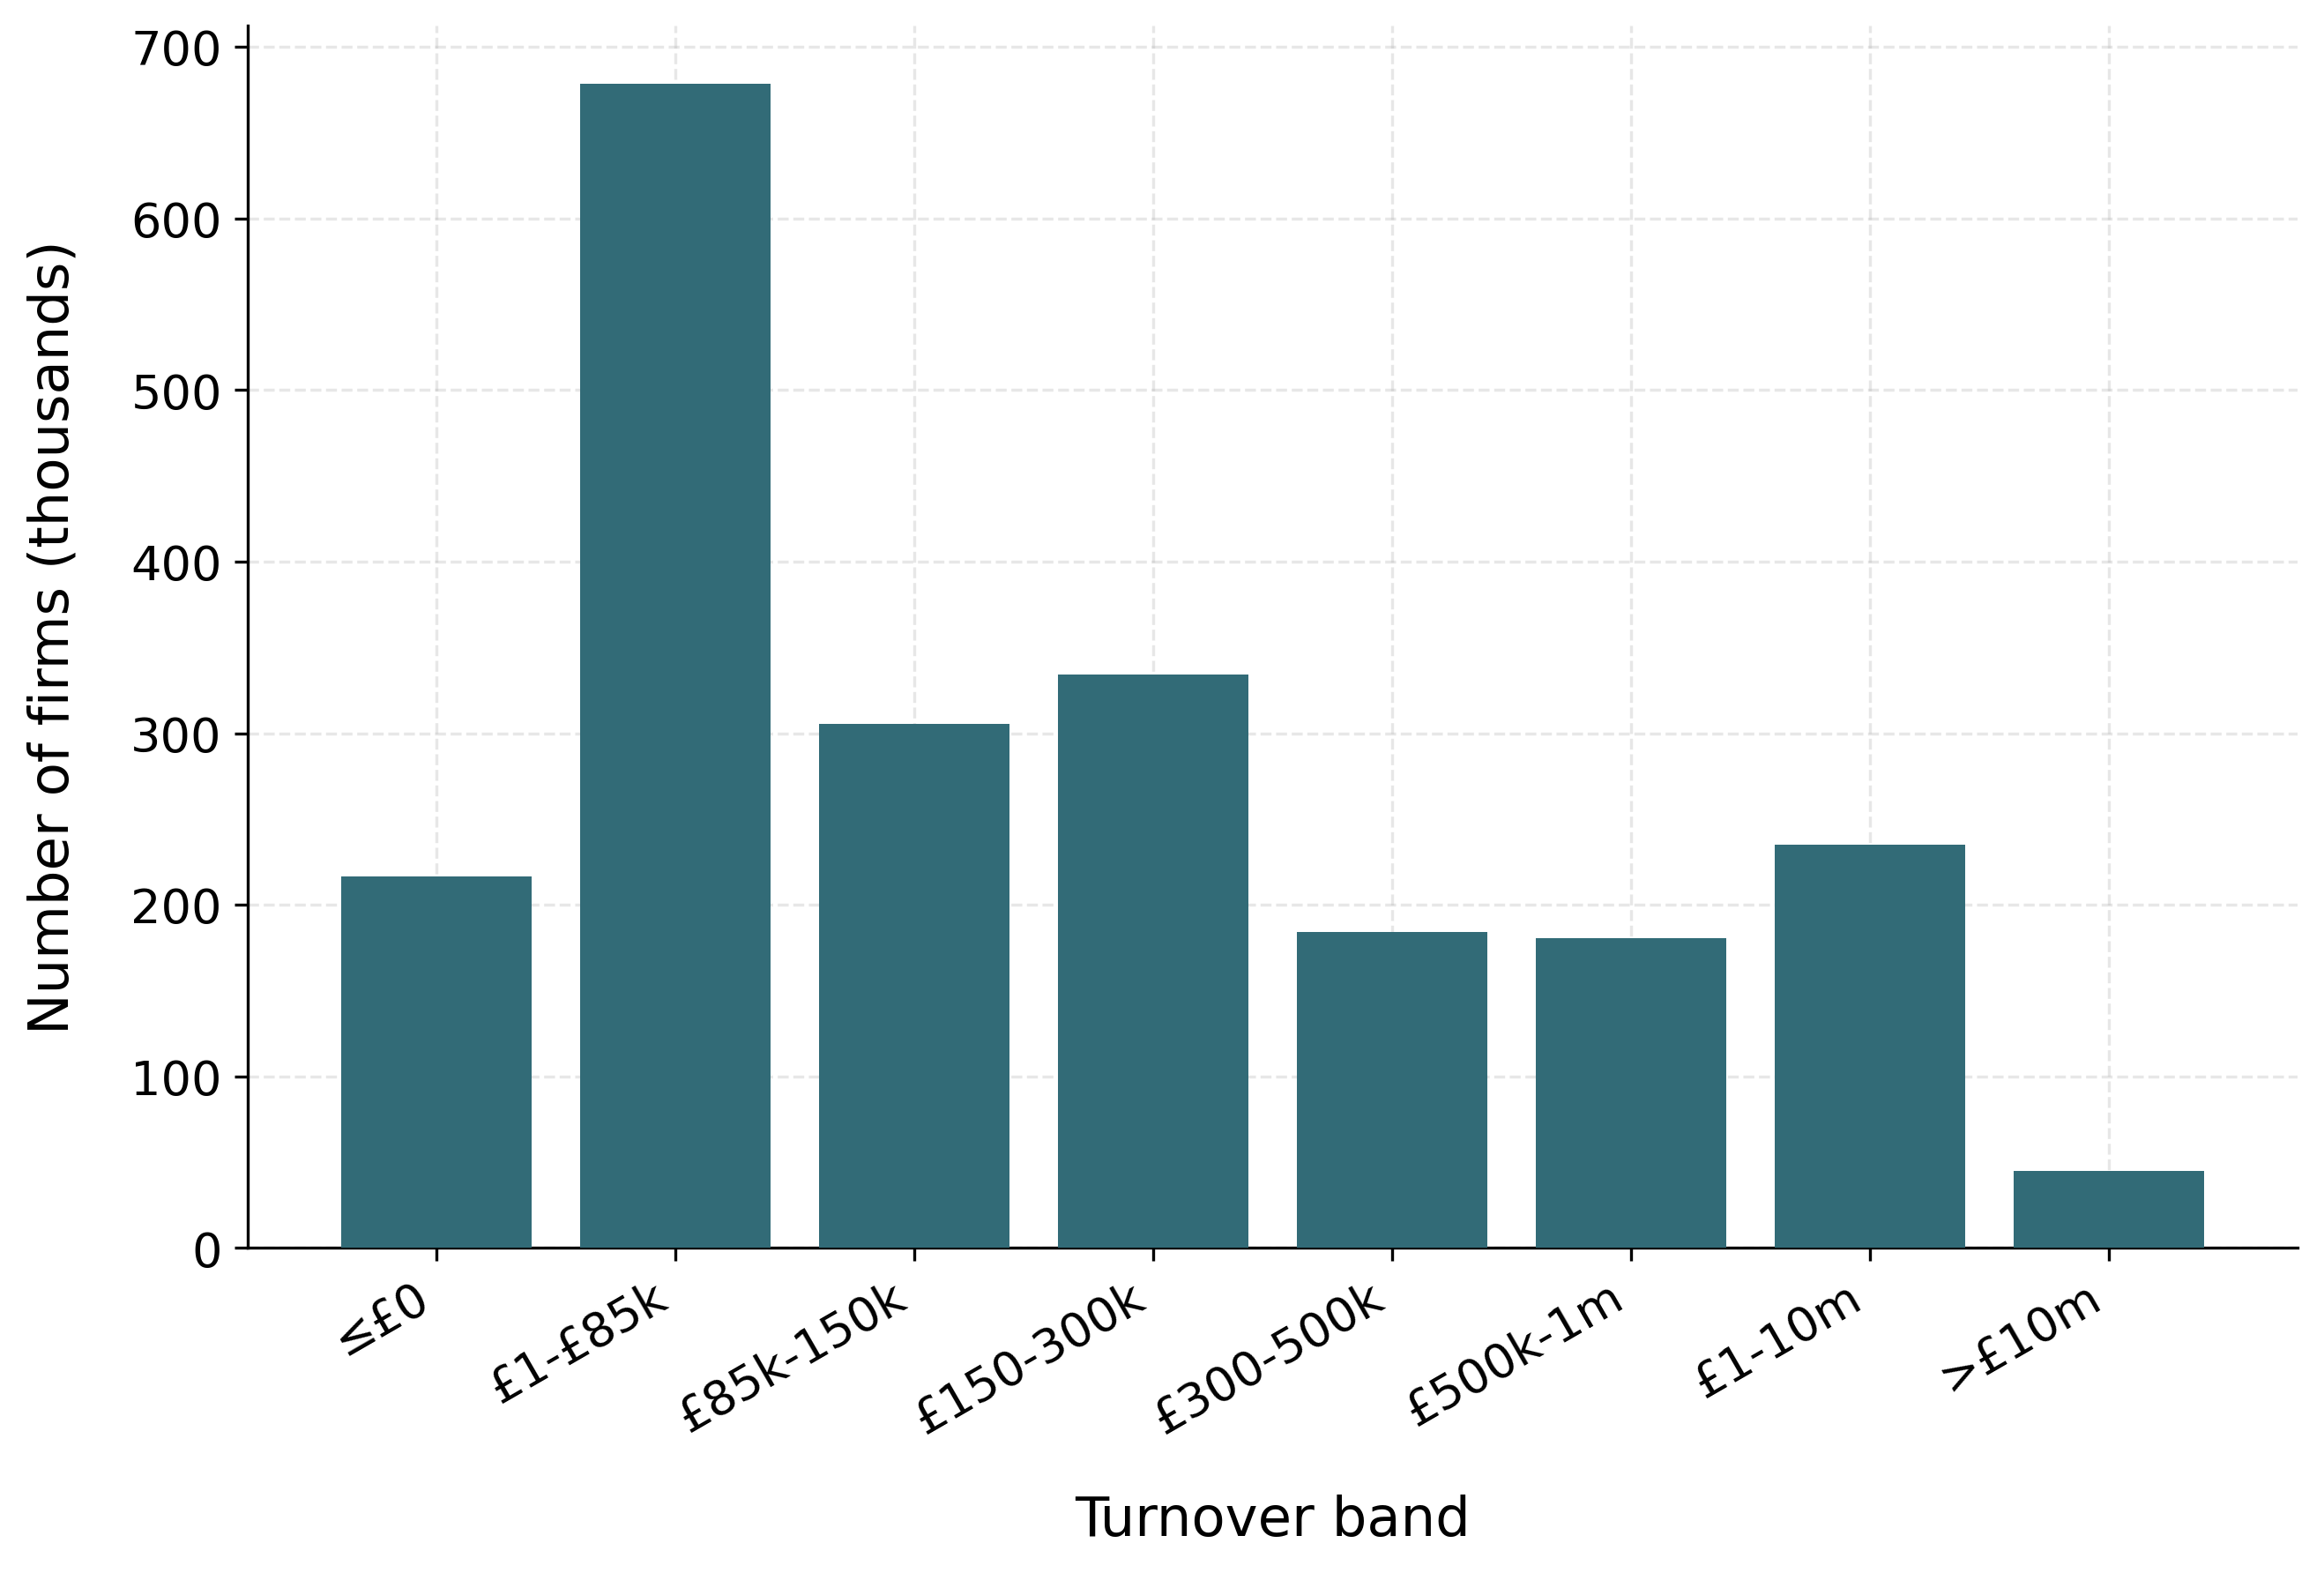
\includegraphics[height=0.50\textheight,width=\linewidth,keepaspectratio]{vat_firms_by_turnover_band_85k.png}\\[0.3em]
    {\scriptsize VAT-registered firms by band (HMRC)}
  \end{minipage}\hfill
  \begin{minipage}[t]{0.32\textwidth}
    \centering
    
\includegraphics[height=0.50\textheight,width=\linewidth,keepaspectratio]{obr_vat_bunching_85k.png}\\[0.3em]
    {\scriptsize Bunching below \pounds85k (OBR, 2023)}
  \end{minipage}
\end{frame}

% --- This paper ---
\begin{frame}{This paper}
  \begin{itemize}\itemsep0.25cm
    \item An \alert{open, reproducible firm-level microsimulation} that costs
      UK VAT threshold reforms on a common static basis.
    \item Built on \alert{synthetic firm microdata} calibrated to published
      HMRC + ONS aggregates --- \alert{released openly} and regenerable under
      any counterfactual schedule.
    \item Prices three reform families --- \alert{level} (move the threshold),
      \alert{shape} (a graduated taper), \alert{rate} (a reduced-rate band) ---
      \alert{three ways}:
      \begin{itemize}\itemsep0.1cm
        \item[1.] \textbf{statically} (mechanical reclassification);
        \item[2.] by the exact, elasticity-free \textbf{dominated-region} distortion each removes;
        \item[3.] \textbf{behaviourally}, conditional on an assumed turnover elasticity $e$.
      \end{itemize}
    \item \alert{Headline:} only the graduated taper removes the notch's
      distortion; raising the threshold is the dearest, least efficient option.
  \end{itemize}
\end{frame}

% --- Literature ---
\begin{frame}{Related literature}
  \begin{itemize}\itemsep0.3cm
    \item \textbf{Bunching / notch methodology} --- source of the
      ``dominated region''
      \begin{itemize}
        \item \citet{saez2010}; \citet{klevenwaseem2013}; \citet{kleven2016}
      \end{itemize}
    \item \textbf{VAT registration threshold (empirical)}
      \begin{itemize}
        \item \citet{liuetal2021} (UK notch, $\sim$43\% voluntary registration);
          \citet{liulockwoodtam2024}; \citet{onji2009}; \citet{asatryanpeichl2017}; \citet{waseem2024}
      \end{itemize}
    \item \textbf{Does bunching identify a structural elasticity?}
      \begin{itemize}
        \item \citet{blomquistetal2021}; \citet{bertanhaetal2023} --- \emph{not} non-parametrically identified
      \end{itemize}
    \item \textbf{Structural models of size-based thresholds}
      \begin{itemize}
        \item \citet{garicano2016}; \citet{gourioroys2014}
      \end{itemize}
  \end{itemize}
\end{frame}

\section{Data and calibration}

% --- Data sources ---
\begin{frame}{Data: synthetic firms calibrated to public aggregates}
  \hypertarget{slide:data}{}
  \begin{itemize}\itemsep0.3cm
    \item \textbf{No open firm-level VAT microdata exist} $\Rightarrow$ build a
      synthetic population calibrated to published aggregates (data year 2023--24).
    \item \textbf{Calibration targets:}
      \begin{itemize}
        \item ONS \emph{UK Business: Activity, Size and Location} --- firm counts by sector $\times$ turnover band
        \item HMRC \emph{VAT Annual Statistics} --- registered counts and net VAT liability by band / sector
      \end{itemize}
    \item \textbf{Scale:} $\approx$\alert{2.94m} firm records, weighted to
      represent $\approx$\alert{2.5m} UK firms.
    \item \textbf{Accuracy:} $\approx$\alert{90\%} across five calibrated dimensions.
    \item Approach mirrors open household tax-benefit microsimulation \citep{policyengine}.
  \end{itemize}
  \begin{textblock*}{8.6cm}(5.4cm,7.95cm)
    \raggedleft
    \hyperlink{slide:generation}{\beamergotobutton{how firms are built}}\quad
    \hyperlink{slide:turnover_fig}{\beamergotobutton{distribution}}
  \end{textblock*}
\end{frame}

% --- Turnover distribution figure ---
\begin{frame}{The calibrated turnover distribution}
  \hypertarget{slide:turnover_fig}{}
  \begin{figure}
    \centering
    
\includegraphics[height=0.62\textheight]{turnover_distribution_85k.png}
  \end{figure}
  \vspace{-0.2cm}
  {\footnotesize Density steps down at the \pounds85{,}000 registration
  threshold and again at the \pounds150{,}000 Flat Rate Scheme ceiling.
  \alert{The step is inherited from coarse HMRC band targets} --- quantified later by a placebo test.}
\end{frame}

\section{Static costing}

% --- Static formula + reform families ---
\begin{frame}{Static costing: mechanical reclassification}
  \begin{block}{Static revenue at threshold $T$}
    \[ R(T) = \sum_i w_i\, v_i\, \mathbf{1}\{y_i \ge T\}. \]
  \end{block}
  \begin{itemize}\itemsep0.2cm
    \item Turnover held fixed $\Rightarrow$ revenue moves \alert{only through
      firms whose registration status flips} (those between the old and new cutoff).
    \item Three reform \alert{levers}, four schedules, all on one base:
      \begin{itemize}
        \item \textbf{Level} --- move the threshold up or down
        \item \textbf{Shape} --- graduated taper, 0\% at \pounds85k $\to$ 20\% at \pounds105k
        \item \textbf{Rate} --- reduced-rate band (10\% or 15\%) in \pounds85k--\pounds105k
      \end{itemize}
    \item For each, recompute $R=\sum_i w_i v_i$ under the new schedule and difference.
  \end{itemize}
\end{frame}

% --- Validation vs HMRC ---
\begin{frame}{Validation: the April-2024 anchor reform}
  \hypertarget{slide:validation}{}
  \begin{columns}[T]
    \begin{column}{0.56\textwidth}
      \begin{figure}
        \centering
        
\includegraphics[width=\linewidth]{vat_threshold_revenue_impact.png}
      \end{figure}
    \end{column}
    \begin{column}{0.44\textwidth}
      \footnotesize
      \begin{itemize}\itemsep0.25cm
        \item Cost the \alert{\pounds85k$\to$\pounds90k} April-2024 rise, my
          estimate vs HMRC's published costing.
        \item \alert{2025--26: \pounds175m vs \pounds185m} --- agree within
          \pounds7--21m per year across the horizon.
        \item Both turn to a small \emph{gain} by 2028--29 as fiscal drag lifts
          the frozen baseline.
        \item Microdata are calibrated to HMRC aggregates $\Rightarrow$ a
          \alert{consistency check}, not out-of-sample validation.
      \end{itemize}
    \end{column}
  \end{columns}
\end{frame}

% --- Threshold sweep ---
\begin{frame}{Static sweep: cost of moving the threshold (2025--26)}
  {\footnotesize Validated on the one move HMRC published, \alert{now sweep the
  whole schedule} --- the same mechanical reclassification at every threshold.}
  \vspace{0.15cm}
  \begin{figure}
    \centering
    
\includegraphics[width=0.46\linewidth]{revenue_impact_2025_26.png}\hfill
    
\includegraphics[width=0.46\linewidth]{firms_impact_2025_26.png}
  \end{figure}
  \vspace{-0.1cm}
  {\footnotesize From a \pounds90k base (\pounds203.8bn), the schedule is
  roughly linear, \alert{$\approx$\pounds150--220m per \pounds5k step}: e.g.\
  \alert{$-$\pounds374m} to raise to \pounds100k, \alert{$+$\pounds665m} to
  lower to \pounds70k. Even a \pounds30k rise to \pounds120k costs $\sim$\pounds1.2bn --- under 0.6\% of the base.}
\end{frame}

% --- Reform menu ---
\begin{frame}{The reform menu, one common base}
  \hypertarget{slide:menu}{}
  \begin{center}
    \renewcommand{\arraystretch}{1.35}
    \begin{tabular}{@{}l l r l@{}}
      \toprule
      \textbf{Reform} & \textbf{Lever} & \textbf{Static} & \textbf{Dominated region} \\
      \midrule
      Raise to \pounds100k     & Level & $-$\pounds508m & relocated \\
      Taper \pounds85--105k    & Shape & $-$\pounds336m & \alert{removed} \\
      Reduced 10\%             & Rate  & $-$\pounds343m & split in two \\
      Reduced 15\%             & Rate  & $-$\pounds171m & split in two \\
      \bottomrule
    \end{tabular}
  \end{center}
  \vspace{0.2cm}
  {\footnotesize Common \pounds85{,}000-notch / \pounds183.6bn 2023--24 base.
  \alert{The level move is the most expensive yet removes no distortion}; the
  taper removes it entirely for less.\\[0.2em]
  \emph{``Split in two''} $=$ a second notch appears where the reduced-rate band
  ends (\pounds105k reverts to 20\%), so the empty band is fragmented, not shrunk.}
  \begin{textblock*}{3cm}(12.6cm,8.4cm)
    \hyperlink{slide:behav_table}{\beamergotobutton{behavioural}}
  \end{textblock*}
\end{frame}

\section{The notch's distortion}

% --- Bunching is mechanical ---
\begin{frame}{Bunching in the synthetic data is mechanical}
  \hypertarget{slide:bunching}{}
  \begin{columns}[T]
    \begin{column}{0.55\textwidth}
      \begin{figure}
        \centering
        
\includegraphics[width=\linewidth,height=0.46\textheight,keepaspectratio]{bunching_analysis_85k.png}
      \end{figure}
      \vspace{-0.2cm}
      {\footnotesize Excess mass over a polynomial no-bunching counterfactual $g$:}
      \[ b=\frac{B(y^{*})}{g(y^{*})}\approx\frac{\Delta y^{*}}{y^{*}},
         \qquad E=\!\!\sum_{\text{window}}\!\big(n_j-c_j\big). \]
    \end{column}
    \begin{column}{0.45\textwidth}
      \footnotesize
      \begin{itemize}\itemsep0.25cm
        \item Reproduced density step: ratio \alert{$b=0.060$} (SE 0.005),
          excess mass \alert{$E=8{,}712$ firms} (SE 662).
        \item \alert{Placebo:} remove the step from the calibration target $\Rightarrow$
          $E$ collapses to \alert{0--99 firms}.
        \item So the step is \alert{inherited from coarse HMRC bands}, not firm
          behaviour --- the generator has no location choice.
        \item Genuine threshold bunching remains the administrative fact of
          \citet{liuetal2021}.
      \end{itemize}
    \end{column}
  \end{columns}
\end{frame}

% --- Dominated region ---
\begin{frame}{The dominated region: an exact, elasticity-free distortion}
  \hypertarget{slide:dominated}{}
  \begin{columns}[T]
    \begin{column}{0.52\textwidth}
      \begin{figure}
        \centering
        
\includegraphics[width=\linewidth,height=0.44\textheight,keepaspectratio]{dynamic_notch_fit_e017.png}
      \end{figure}
      \vspace{-0.15cm}
      {\footnotesize The notch in the firm's profit:}
      \[ \pi(y)=\begin{cases} y-c(y), & y<T^{*},\\[1pt]
                 (1-\tau)\,y-c(y), & y\ge T^{*}.\end{cases} \]
    \end{column}
    \begin{column}{0.48\textwidth}
      \footnotesize
      \begin{itemize}\itemsep0.25cm
        \item At $T^{*}$, profit jumps \emph{down} by $\tau T^{*}=\pounds17{,}000$
          --- VAT on turnover already earned.
        \item The \alert{dominated region} is the band just above $T^{*}$ where
          no firm locates (strictly worse than at $T^{*}$):
          \[ a = T^{*}\frac{\tau}{1-\tau} = \alert{\pounds21{,}250}. \]
        \item Interval \alert{(\pounds85{,}000, \pounds106{,}250)},
          $\approx$\alert{137{,}000} weighted firms.
        \item Depends on $\tau$ and $T^{*}$ \alert{alone} --- no elasticity, no
          cost specification. An order of magnitude wider than a kink's $\sim$\pounds1k.
      \end{itemize}
    \end{column}
  \end{columns}
\end{frame}

% --- How reforms change it ---
\begin{frame}{Which reforms actually shrink the band?}
  \begin{itemize}\itemsep0.3cm
    \item \textbf{Raise the threshold} --- \alert{relocates} the \pounds21{,}250
      band unchanged to the new cutoff.
    \item \textbf{Banded reduced rate} --- does \alert{not} shrink it. Lowers the
      single notch ($\pounds17{,}000 \to \pounds12{,}750$ at 15\%) but adds a
      \alert{secondary notch} where the band reverts at \pounds105k:
      \[ a' = T_1\frac{\tau-r}{1-\tau}; \qquad
         a+a' = \pounds21{,}562\ (15\%),\ \ \pounds22{,}569\ (10\%). \]
      It \alert{splits one wide empty band into two}, not shrinks it.
    \item \textbf{Graduated taper} --- continuous, \alert{no notch and no
      dominated region}: it removes the distortion entirely.
  \end{itemize}
  \vspace{0.2cm}
  \begin{center}
    \alert{Only the taper removes the distortion --- and for less (\pounds336m).}
  \end{center}
\end{frame}

\section{Behavioural layer}

% --- Behavioural ---
\begin{frame}{The firm's problem: VAT on \emph{value added} (formulation A)}
  \begin{columns}[T]
    \begin{column}{0.5\textwidth}
      \scriptsize
      A firm of ability $n$ chooses turnover $y$ to maximise
      \[ \pi(y)=(1-\delta)\bigl(1-\tau f(y)\bigr)\,y-C(y;n,e). \]
      \begin{itemize}\itemsep0.12cm
        \item VAT falls on \alert{value added} $(1-\delta)y$, not whole turnover;
          $\delta$ is the firm's \alert{deductible-input share}.
        \item $C$ is the firm's \alert{own-factor cost} (labour, capital): inputs
          $\delta y$ are already netted by $(1-\delta)$, so reading $C$ as total
          cost would \alert{double-count} them.
        \item Optimum $y^{\star}=n\bigl[(1-\delta)(1-\tau)\bigr]^{e}$. $\delta$ is
          parametric for now --- ONS Supply--Use value-added shares to come.
      \end{itemize}
    \end{column}
    \begin{column}{0.5\textwidth}
      \begin{figure}\centering
        
\includegraphics[width=\linewidth,height=0.66\textheight,keepaspectratio]{formulation_a_optima.png}
      \end{figure}
      \vspace{-0.1cm}
      {\scriptsize Higher $\delta$ scales the curve down and pulls the registered
      optimum toward the threshold (eventually tipping to bunching).}
    \end{column}
  \end{columns}
\end{frame}

\begin{frame}{Behavioural layer: conditional on an assumed elasticity}
  \hypertarget{slide:behavioural}{}
  \begin{columns}[T]
    \begin{column}{0.54\textwidth}
      \begin{figure}
        \centering
        
\includegraphics[width=\linewidth,height=0.46\textheight,keepaspectratio]{dynamic_cost_vs_elasticity.png}
      \end{figure}
      \vspace{-0.15cm}
      {\footnotesize Each firm rescales turnover under the reform:}
      \[ y_i^{\star}=y_i\!\left(\frac{1-\tau_{\text{reform}}}{1-\tau_{\text{base}}}\right)^{\!e},
         \qquad \frac{\partial\ln y}{\partial\ln(1-\tau)}=e. \]
    \end{column}
    \begin{column}{0.46\textwidth}
      \scriptsize
      \begin{itemize}\itemsep0.1cm
        \item Iso-elastic simulator (value-added base, formulation~A)
          re-optimises each firm (left); the elasticity $e$ is \alert{assumed},
          not identified.
        \item Sweep $e\in\{0.05,0.17,0.32\}$. At \alert{$e=0.17$}
          base-broadening offsets much of each static loss:
          \begin{itemize}\itemsep0.02cm
            \item raise to \pounds100k: \pounds508m $\to$ \alert{\pounds292m}
            \item 10\% band: \pounds343m $\to$ \alert{\pounds273m}
            \item 15\% band: \pounds171m $\to$ \alert{\pounds135m}
          \end{itemize}
        \item Static cost is the $e\to0$ limit; \alert{only $e=0.05$ has an
          external anchor} \citep{klevenwaseem2013}.
        \item Taper \alert{excluded}: its marginal-rate channel is not
          credibly identified iso-elastically.
      \end{itemize}
    \end{column}
  \end{columns}
\end{frame}

\section{Conclusion}

\begin{frame}{Conclusion}
  \footnotesize
  \begin{itemize}\itemsep0.12cm
    \item \alert{What this is:} an open, reproducible firm-level microsimulation
      that models the UK VAT threshold as a turnover-tax notch on synthetic firm
      data, and prices level / shape / rate reforms \alert{three ways}.
    \item \alert{Static:} reproduces HMRC's anchor costing within $\sim$\pounds10m;
      raising to \pounds100k costs \pounds508m, the taper \pounds336m.
    \item \alert{Distortion:} the dominated region $a=\pounds21{,}250$ is exact and
      elasticity-free --- \alert{only the taper removes it}; the level move merely
      relocates it; a reduced rate splits it in two.
    \item \alert{Transparency:} synthetic bunching is mechanical (placebo:
      $8{,}712 \to \sim99$ firms) --- no elasticity is read off the data.
    \item \alert{Behavioural offsets} are conditional on assumed $e$; the static
      cost and dominated region are the elasticity-free anchors.
    \item \alert{Next:} identify $e$ from administrative microdata; add welfare /
      MVPF accounting; sectoral incidence.
  \end{itemize}
\end{frame}

{
\setbeamercolor{background canvas}{bg=pelight}
\begin{frame}[plain,noframenumbering]
  \vfill
  \begin{columns}[c]
    \begin{column}{0.57\textwidth}
      \raggedright
      {\fontsize{22}{26}\selectfont\bfseries\color{pedarkteal}Thank you!\par}
      \vspace{0.35cm}
      {\color{peteal}\rule{0.55\textwidth}{1pt}}\par
      \vspace{0.75cm}
      {\color{pedarkteal}\faGlobe~~\texttt{policyengine.org}\par}
      \vspace{0.28cm}
      {\color{pedarkteal}\faEnvelope~~\texttt{vahid@policyengine.org}\par}
    \end{column}
    \begin{column}{0.40\textwidth}
      \centering
      \qrcode[height=3cm]{https://firm-microsim-paper.vercel.app/}\\[0.5em]
      {\footnotesize\color{pegray}Scan: paper, data \& code\par}
    \end{column}
  \end{columns}
  \vfill
\end{frame}
}

% =================================================================
%                          APPENDIX
% =================================================================
\appendix

% --- Generation (moved to appendix; linked from the Data slide) ---
\begin{frame}{Appendix: how the synthetic firms are built}
  \hypertarget{slide:generation}{}
  \footnotesize
  \begin{itemize}\itemsep0.25cm
    \item Draw firms by sector $\times$ ONS turnover band; turnover smoothed within band:
      \[ y_i = \underline{b} + (\overline{b}-\underline{b})\,u_i + \varepsilon_i,
         \quad u_i\sim\mathcal{U}(0,1),\ \varepsilon_i\sim\mathcal{N}(0,\sigma_b^2). \]
    \item Input share $x_i=\rho_i y_i$ ($\rho_i\in[0.6,1.5]$, rescaled Beta) $\Rightarrow$
      net VAT base \alert{$v_i = y_i - x_i$}.
    \item Each firm gets a strictly positive weight \alert{$w_i = e^{\theta_i}$};
      weighted target $\widehat{T}_k(\theta)=\sum_i a_{ki}w_i$.
    \item Fit $\theta$ by \alert{gradient descent} on a symmetric relative-error loss:
      \[ L(\theta)=\tfrac{1}{K}\textstyle\sum_k \lambda_k
         \min\!\big\{(\widehat{T}_k/T_k-1)^2,\,(T_k/\widehat{T}_k-1)^2\big\}
         + \tfrac{\alpha}{N}\sum_i|\theta_i|. \]
    \item \alert{The threshold is a generator parameter}: every counterfactual ---
      higher cutoff, taper, reduced rate --- regenerates a fresh, internally
      consistent population.
  \end{itemize}
  \back{slide:data}
\end{frame}

\begin{frame}{Appendix: notch vs.\ kink}
  \hypertarget{slide:notch_def}{}
  \begin{itemize}\itemsep0.35cm
    \item A \alert{kink} taxes only the turnover \emph{above} the threshold ---
      the marginal rate jumps, but liability is continuous.
    \item A \alert{notch} taxes the firm's \emph{entire} turnover once it
      registers --- liability jumps discretely by $\tau T^{*}=\pounds17{,}000$.
    \item The UK VAT threshold is a notch $\Rightarrow$ a strict
      \alert{dominated region} exists (no firm should locate just above $T^{*}$),
      whereas a kink leaves only a $\sim$\pounds1k smoothed gap.
    \item This is why the distortion can be measured \alert{exactly and without
      any elasticity}.
  \end{itemize}
  \back{slide:motivation}
\end{frame}

\begin{frame}{Appendix: behavioural costs across $e$}
  \hypertarget{slide:behav_table}{}
  \begin{center}
    \footnotesize
    \renewcommand{\arraystretch}{1.3}
    \begin{tabular}{@{}l r r r r@{}}
      \toprule
      \textbf{Reform} & \textbf{Static ($e{=}0$)} & $e{=}0.05$ & $e{=}0.17$ & $e{=}0.32$ \\
      \midrule
      Raise to \pounds100k & $-$\pounds508m & $-$\pounds444m & $-$\pounds292m & $-$\pounds111m \\
      Reduced 10\% band    & $-$\pounds343m & $-$\pounds322m & $-$\pounds273m & $-$\pounds210m \\
      Reduced 15\% band    & $-$\pounds171m & $-$\pounds160m & $-$\pounds135m & $-$\pounds107m \\
      \bottomrule
    \end{tabular}
  \end{center}
  \vspace{0.25cm}
  {\footnotesize A larger $e$ makes every flat reform cheaper (base-broadening).
  The graduated taper is omitted --- its base-broadening and marginal-rate
  channels cannot both be netted in the iso-elastic cost. The $e\to0$ limit
  reproduces the static costs to within $\sim$\pounds1m.}
  \back{slide:menu}
\end{frame}

\begin{frame}{Appendix: secondary-notch arithmetic (reduced rate)}
  \hypertarget{slide:secondary}{}
  \footnotesize
  A reduced rate $r$ in $[T^{*},T_1]$ with $T_1=\pounds105{,}000$:
  \begin{itemize}\itemsep0.3cm
    \item \textbf{Primary} notch shrinks: jump $rT^{*}$, width
      $a = T^{*}\dfrac{r}{1-r}$ \;=\; \pounds15{,}000 (15\%), \pounds9{,}444 (10\%).
    \item \textbf{Secondary} notch at the band top, where rate reverts to $\tau$:
      jump $(\tau-r)T_1=\pounds5{,}250$ (15\%), width
      $a' = T_1\dfrac{\tau-r}{1-\tau}$ \;=\; \pounds6{,}562 (15\%), \pounds13{,}125 (10\%).
    \item \textbf{Total} dominated width $a+a' = \pounds21{,}562$ (15\%),
      $\pounds22{,}569$ (10\%) --- both marginally \emph{above} the
      \pounds21{,}250 baseline.
  \end{itemize}
  \begin{center}\alert{The reduced rate splits the empty band; it does not shrink it.}\end{center}
  \back{slide:dominated}
\end{frame}

\begin{frame}{Appendix: limitations and future work}
  \begin{itemize}\itemsep0.25cm
    \item \textbf{Value added, parametric $\delta$} --- the behavioural simulator
      now taxes \emph{value added} $(1-\delta)y$ (formulation~A), but $\delta$ is
      parametric, not yet measured firm by firm (ONS Supply--Use to come); the
      dominated region still uses the statutory-rate notch, and $\sim$43\% of
      below-threshold firms register voluntarily \citep{liuetal2021}, which the
      model abstracts from.
    \item \textbf{Partial efficiency metric} --- dominated-region width indexes
      misallocation only, omitting compliance-cost savings \citep{keenmintz2004};
      a full welfare / MVPF accounting is needed.
    \item \textbf{Aggregate only} --- no sectoral incidence (VAT liability by
      sector excluded from the optimiser).
    \item \textbf{Synthetic, partial-equilibrium} --- abstracts from price
      pass-through; no genuine firm location choice.
  \end{itemize}
\end{frame}

\end{document}
